% Drawing 154/07-5 -- folder 154, batch 07, archive page 127 (PDF page 128).
% Transcription: dessins en couleur, sans texte : une colonne de trois disques tangents (bleus et au crayon) traversés par une même pseudo-droite orange ; un disque rempli de pseudo-droites orange, entouré d'un cercle vert en tirets, tangent à un cercle vert vide ; un disque aux pseudo-droites orange dont le bord porte de petites encoches bleues en demi-cercle ; un disque vert et bleu rempli de pseudo-droites orange ; un disque au crayon ; un polygone au crayon avec une étoile de flèches orange et de rayons bleus
% Kind: column of tangent disks crossed by one pseudoline; disks with arrangements; tangent empty circle; star of arrows. Method 2 (schematic redraw from the facsimile). Status: partial.
% Notes: Colour drawings without text, over an upside-down job log (not reproduced), read from the page view: a column of three tangent disks (blue and pencil) crossed by one orange pseudoline; a disk filled with orange pseudolines surrounded by a dashed green circle, tangent to an empty light green circle; a disk with orange pseudolines whose rim carries small blue and green bumps; a disk with orange pseudolines and green rim; a pencil disk with crossing lines; a pencil star of orange arrows in a pencil polygon; a pencil stroke at the left. Arrangements schematic.
% Coordinates: 1 unit = 1 mm = 1/100 of the crop width (bbox in page fractions: [0.157, 0.092, 0.896, 0.451]).
% Redrawn by Claude (claude-opus-5-5), issue #73, 2026-11-07; not checked by a human; not compiled (no TeX in the session).
% Rights: reproduces part of the work -- behind RENDER_TRANSCRIPTS, never published by itself.
\documentclass[tikz,border=3pt]{standalone}
\usepackage{amsmath,amssymb}
\usetikzlibrary{patterns,arrows.meta}
\tikzset{Or/.style={orange!90!black}, Ye/.style={yellow!80!orange}, Lg/.style={green!60!black!70}, Dg/.style={green!45!black}, Br/.style={brown!80!black}, Rd/.style={red!85!black}, Bl/.style={blue!70!black}, Gy/.style={black!40}, pencil/.style={black!45}, struck/.style={black!35}, mark/.style={circle,draw,inner sep=1.3pt}, pt/.style={circle,fill,inner sep=0.9pt}, opt/.style={circle,draw,fill=white,inner sep=1.1pt}}
\begin{document}
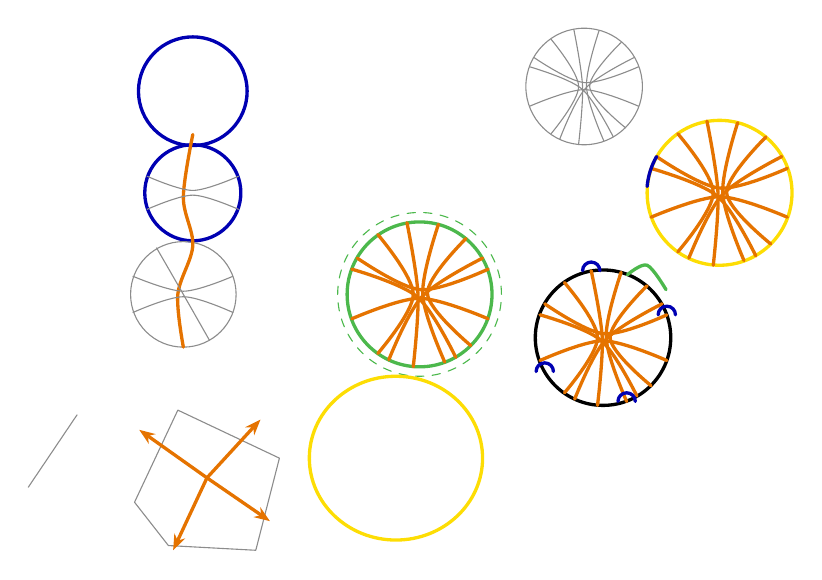
\begin{tikzpicture}[x=1mm,y=1mm,line cap=round,line join=round,font=\scriptsize]
\draw[Bl,very thick] (22.1,-9.8) circle[radius=6.9];
\draw[Bl,very thick] (22.1,-22.7) circle[radius=6.1];
\draw[pencil] (20.9,-35.6) circle[radius=6.7];
\draw[Or,very thick] plot[smooth, tension=0.55] coordinates {(22.1,-15.3) (20.9,-23.3) (22.1,-29.4) (20.2,-35.6) (20.9,-42.3)};
\draw[pencil] plot[smooth, tension=0.55] coordinates {(16.3,-20.6) (22.1,-22.4) (27.9,-20.6)};
\draw[pencil] plot[smooth, tension=0.55] coordinates {(16.3,-24.8) (22.1,-23) (27.9,-24.8)};
\draw[pencil] plot[smooth, tension=0.55] coordinates {(14.5,-33.3) (20.9,-35.2) (27.2,-33.3)};
\draw[pencil] plot[smooth, tension=0.55] coordinates {(14.5,-37.9) (20.9,-35.9) (27.2,-37.9)};
\draw[pencil] plot[smooth, tension=0.55] coordinates {(17.5,-29.7) (20.9,-35.6) (24.2,-41.4)};
\draw[Lg,very thick] (50.9,-35.6) circle[radius=9.2];
\draw[Lg,dashed] (50.9,-35.6) circle[radius=10.4];
\draw[Or,very thick] plot[smooth, tension=0.55] coordinates {(49.3,-26.5) (50.7,-35.6) (50.1,-44.8)};
\draw[Or,very thick] plot[smooth, tension=0.55] coordinates {(53.3,-26.7) (51.3,-35.6) (54.1,-44.2)};
\draw[Or,very thick] plot[smooth, tension=0.55] coordinates {(45.6,-28) (50.1,-35.6) (45.6,-43.1)};
\draw[Or,very thick] plot[smooth, tension=0.55] coordinates {(56.8,-28.5) (51.9,-35.5) (57.4,-42.1)};
\draw[Or,very thick] plot[smooth, tension=0.55] coordinates {(43,-31) (51,-35) (59.6,-32.4)};
\draw[Or,very thick] plot[smooth, tension=0.55] coordinates {(42.3,-38.7) (50.9,-36.1) (59.6,-38.7)};
\draw[Or,very thick] plot[smooth, tension=0.55] coordinates {(58.9,-31) (51.2,-35.9) (47,-43.9)};
\draw[Or,very thick] plot[smooth, tension=0.55] coordinates {(42.3,-32.4) (50.6,-35.9) (55.5,-43.6)};
\draw[Ye,very thick] (47.9,-56.4) ellipse[x radius=11, y radius=10.4];
\draw[very thick] (74.2,-41.1) circle[radius=8.6];
\draw[Or,very thick] plot[smooth, tension=0.55] coordinates {(72.7,-32.6) (74.1,-41.1) (73.5,-49.7)};
\draw[Or,very thick] plot[smooth, tension=0.55] coordinates {(76.5,-32.8) (74.6,-41.1) (77.2,-49.2)};
\draw[Or,very thick] plot[smooth, tension=0.55] coordinates {(69.3,-34.1) (73.5,-41.1) (69.3,-48.1)};
\draw[Or,very thick] plot[smooth, tension=0.55] coordinates {(79.8,-34.5) (75.1,-41.1) (80.3,-47.2)};
\draw[Or,very thick] plot[smooth, tension=0.55] coordinates {(66.8,-36.8) (74.3,-40.6) (82.3,-38.2)};
\draw[Or,very thick] plot[smooth, tension=0.55] coordinates {(66.2,-44) (74.2,-41.5) (82.3,-44)};
\draw[Or,very thick] plot[smooth, tension=0.55] coordinates {(81.7,-36.8) (74.5,-41.4) (70.6,-48.9)};
\draw[Or,very thick] plot[smooth, tension=0.55] coordinates {(66.2,-38.2) (73.9,-41.4) (78.5,-48.5)};
\draw[Bl,very thick] (73.8,-32.6) arc[start angle=0, end angle=180, x radius=1.1, y radius=1.1];
\draw[Bl,very thick] (67.9,-45.4) arc[start angle=0, end angle=180, x radius=1.1, y radius=1.1];
\draw[Bl,very thick] (78.3,-49.2) arc[start angle=0, end angle=180, x radius=1.1, y radius=1.1];
\draw[Bl,very thick] (83.4,-38.2) arc[start angle=0, end angle=180, x radius=1.1, y radius=1.1];
\draw[Lg,very thick] plot[smooth, tension=0.55] coordinates {(77.3,-33.1) (79.8,-31.9) (82.2,-35)};
\draw[Ye,very thick] (89,-22.7) circle[radius=9.2];
\draw[Or,very thick] plot[smooth, tension=0.55] coordinates {(87.4,-13.6) (88.8,-22.7) (88.2,-31.9)};
\draw[Or,very thick] plot[smooth, tension=0.55] coordinates {(91.3,-13.8) (89.4,-22.7) (92.1,-31.3)};
\draw[Or,very thick] plot[smooth, tension=0.55] coordinates {(83.7,-15.2) (88.2,-22.7) (83.7,-30.2)};
\draw[Or,very thick] plot[smooth, tension=0.55] coordinates {(94.9,-15.6) (89.9,-22.7) (95.5,-29.2)};
\draw[Or,very thick] plot[smooth, tension=0.55] coordinates {(81,-18.1) (89,-22.1) (97.6,-19.6)};
\draw[Or,very thick] plot[smooth, tension=0.55] coordinates {(80.3,-25.8) (89,-23.2) (97.6,-25.8)};
\draw[Or,very thick] plot[smooth, tension=0.55] coordinates {(96.9,-18.1) (89.3,-23) (85.1,-31)};
\draw[Or,very thick] plot[smooth, tension=0.55] coordinates {(80.3,-19.6) (88.7,-23.1) (93.6,-30.7)};
\draw[Bl,very thick] (81,-18.1) arc[start angle=150, end angle=175, x radius=9.2, y radius=9.2];
\draw[pencil] (71.8,-9.2) circle[radius=7.4];
\draw[pencil] plot[smooth, tension=0.55] coordinates {(70.5,-2) (71.6,-9.2) (71.1,-16.5)};
\draw[pencil] plot[smooth, tension=0.55] coordinates {(73.7,-2.1) (72.1,-9.2) (74.3,-16.1)};
\draw[pencil] plot[smooth, tension=0.55] coordinates {(67.6,-3.2) (71.1,-9.2) (67.6,-15.2)};
\draw[pencil] plot[smooth, tension=0.55] coordinates {(76.5,-3.6) (72.5,-9.2) (77,-14.4)};
\draw[pencil] plot[smooth, tension=0.55] coordinates {(65.4,-5.5) (71.8,-8.7) (78.7,-6.7)};
\draw[pencil] plot[smooth, tension=0.55] coordinates {(64.9,-11.7) (71.8,-9.6) (78.7,-11.7)};
\draw[pencil] plot[smooth, tension=0.55] coordinates {(78.2,-5.5) (72,-9.4) (68.7,-15.9)};
\draw[pencil] plot[smooth, tension=0.55] coordinates {(64.9,-6.7) (71.5,-9.5) (75.5,-15.6)};
\draw[pencil] (14.7,-62) -- (20.2,-50.3) -- (33.1,-56.4) -- (30.1,-68.1) -- (19,-67.5) -- cycle;
\draw[Or,very thick,-{Stealth[length=2mm]}] (23.9,-58.9) -- (15.3,-52.8);
\draw[Or,very thick,-{Stealth[length=2mm]}] (23.9,-58.9) -- (30.7,-51.5);
\draw[Or,very thick,-{Stealth[length=2mm]}] (23.9,-58.9) -- (31.9,-64.4);
\draw[Or,very thick,-{Stealth[length=2mm]}] (23.9,-58.9) -- (19.6,-68.1);
\draw[pencil] (1.2,-60.1) -- (7.4,-50.9);
\end{tikzpicture}
\end{document}
